\documentclass[review]{elsarticle}

\usepackage{hyperref}

\journal{Computers in Biology and Medicine}

\usepackage{graphicx}
\usepackage[utf8]{inputenc}
\usepackage[]{caption}
\usepackage{hyperref}
\usepackage[]{subcaption}
\usepackage{amsmath}
\usepackage{enumerate}
\usepackage{algorithm}
\usepackage{algorithmicx}
\usepackage{algpseudocode}


\newcommand{\argmin}{\operatornamewithlimits{arg\ min}}
\newcommand{\argmax}{\operatornamewithlimits{arg\ max}}
\newcommand{\defeq}{\stackrel{\triangle}{=}} %dodao
\renewcommand{\vec}[1]{\mathbf{#1}} %dodao
\newcommand{\operator}[2]{\mathop{#1}_{#2}} %dodao
\newtheorem{mydef}{Definition}%dodao

\linespread{1.5}

\begin{document}

\begin{frontmatter}

\title{Left Atrial Appendage Segmentation from 3D CCTA Images for Occluder Placement Procedure}

\author[ferit]{Hrvoje Leventić\corref{cor1}}
\ead{hrvoje.leventic@ferit.hr}

\author[bd]{Danilo Babin}

\author[ikv]{Lazar Velicki}
\author[uzgent]{Daniel Devos}
\author[ferit]{Irena Galić}
\author[ftn]{Vladimir Zlokolica}
\author[ferit]{Krešimir Romić}
\author[ap]{Aleksandra Pižurica}



\cortext[cor1]{Corresponding author}

\address[ferit]{Faculty of Electrical Engineering, Computer Science and Information Technology, 
University J. J. Strossmayer Osijek, Croatia}
\address[bd]{imec-TELIN-IPI, Faculty of Engineering and Architecture, Ghent University, Belgium}
\address[ikv]{Faculty of Medicine, University of Novi Sad, Serbia; and Institute for Cardiovascular Diseases of Vojvodina, Sremska Kamenica, Serbia}
\address[uzgent]{University Hospital Ghent, Ghent University, Belgium}
\address[ftn]{Faculty of Technical Sciences, University of Novi Sad, Serbia}
\address[ap]{TELIN-IPI, Faculty of Engineering and Architecture, Ghent University - imec, Belgium}


\begin{abstract}
    \paragraph{\textbf{Background}}
    Percutaneous left atrial appendage (LAA) closure (placement of an
    occluder to close the appendage) is a novel procedure for stroke prevention in
    patients suffering from atrial fibrillation. 
    The closure procedure planning requires accurate LAA
    measurements which can be obtained from computed tomography (CT) images. \\
    \paragraph{\textbf{Method}}
    We propose a novel semi-automatic LAA
    segmentation method from 3D coronary CT angiography (CCTA) images. The
    method segments the LAA, proposes the location for the occluder placement
    (a delineation plane between the left atrium and LAA) and calculates
    measurements needed for closure procedure planning. 
    The method requires only two
    inputs from the user: a threshold value and a single seed point inside the
    LAA. 
    Proposed location of the delineation plane can be intuitively corrected if necessary. 
    Measurements are calculated from the segmented LAA according to the final
    delineation plane.  \\
    \paragraph{\textbf{Results}}
    Performance of the proposed method is validated on
    17 CCTA images, manually segmented by two medical doctors. 
    We achieve the average dice coefficient overlap of 92.52\% and 91.63\%
    against the ground truth segmentations.  The average dice coefficient overlap
    between the two ground truth segmentations is 92.66\%. 
    Our proposed LAA orifice localization is
    evaluated against the desired location of the LAA orifice determined by the
    expert. The average distance between our proposed location and the desired
    location is 2.51 mm. \\
    \paragraph{\textbf{Conclusion}}
    Segmentation results show high correspondence to the ground truth segmentations. 
    The occluder placement method shows high accuracy which indicates potential in clinical
    procedure planning.\\
\end{abstract}

\begin{keyword}
Left atrial appendage \sep image segmentation \sep  image analysis \sep 
      left atrial appendage occlusion \sep left atrial appendage closure 
\end{keyword}

\end{frontmatter}


\section{Introduction}
\label{intro}

Survey performed by World Health Organization
\cite{worldhealthorganization2017_top10causes} has identified stroke as the
second leading global cause of death with over 6 million deaths in 2015.  The
risk of stroke drastically increases in patients suffering from atrial
fibrillation (AF) \cite{korhonen2015_LeftAtrialAppendage}. 
With atrial fibrillation, the normal regular rhythm of the heart becomes
irregular, due to disorganized electrical signals in the upper heart chambers,
called the atria. This chaotic electrical activity causes asynchronous
contractions of the atria, which do not allow the heart chambers to fill and
empty properly. Without effective blood pumping, the blood can sometimes pool
in the heart and form a blood clot, i.e.
thrombus, and it is this clotting that increases the risk of a stroke. Pieces
can break off from a clot, forming thromboemboli, which can be passed from one chamber to the next
and then end up in the brain arteries causing a stroke.
Atrial fibrillation is a cardiac disease shown to be responsible for almost
20\% of all strokes \cite{budge2008_Analysisvivoleft} and the majority of
cardioembolic strokes \cite{korhonen2015_LeftAtrialAppendage}.  The vast
majority of cardioembolic strokes are the result of cardiac thromboemboli
formed in the LAA
\cite{blackshear1996_Appendageobliterationreduce,goldman1999_Pathophysiologiccorrelatesthromboembolism}.
Estimates show that over 33 million people worldwide suffer from atrial
fibrillation \cite{chugh2013_WorldwideEpidemiologyAtrial}.

Left atrial appendage closure is a stroke prevention method for patients with
AF
 \cite{panaich2017_LeftAtrialAppendage}. The closure
procedure demonstrated non-inferiority to anticoagulation therapy for stroke
prevention \cite{holmes2015_LeftAtrialAppendage,reddy2013_LeftAtrialAppendage}
while avoiding most of the contraindications associated with the
anticoagulation therapy.  The procedure is performed by percutaneously
deploying the occluder device to the neck of the LAA and stopping the blood
flow between left atrium (LA) and LAA, thus preventing the formed trombii from
leaving the LAA and causing stroke. Closure devices are available in
several predefined sizes and for each patient an appropriately sized device has
to be selected. Selection of the correct size of the occluder requires
accurate measurements of the LAA. Coronary CT angiography images (CCTA)
have shown to be superior to other imaging modalities
\cite{saw2016_ComparingMeasurementsCT,goitein2017_CardiacCTAngiography,wunderlich2015_PercutaneousInterventionsLeft,cabrera2014_Leftatrialappendage}.
The work of \cite{cabrera2014_Leftatrialappendage} presents the complete list
of anatomic and imaging landmarks that determine the feasibility of closure
procedure. The most important measurements for correct occluder placement are:
diameter (circumference) of the orifice, shape of the orifice, LAA 
volume and type of the LAA morphology.  These  measurements can be accurately
performed using CCTA image segmentation, analysis and visualization. 


Vast majority of LAA segmentation and analysis studies determine the required
anatomical measurements manually.  Two most often used approaches are: manual
measurements directly from original images
\cite{saw2016_ComparingMeasurementsCT} and measurements from manually segmented
3D volume
\cite{song2016_MorphologicAssessmentLeft,otton2015_LeftAtrialAppendage}.
Manual 3D segmentation is a time-consuming and error prone process, where
segmentation is performed slice-by-slice with a paintbrush tool
\cite{otton2015_LeftAtrialAppendage}. Additionally, 3D segmentation can be
performed using interactive guided segmentation methods. Such methods improve
the segmentation speed but still require time for manual corrections of
segmentation leaks \cite{song2016_MorphologicAssessmentLeft}.  The standard
region growing methods for guided interactive segmentation all suffer from
segmentation leaks due to the inhomogeneous distribution of contrast agent in
the appendage and proximity of highly-contrasted surrounding vessels. In other
words, a threshold value that will accurately isolate the LAA region (so that
no surrounding structures are included) will consequently result in an
under-segmented LAA. On the other hand, a threshold value that will allow for
the whole LAA region to be segmented, will also produce an over-segmentation
due to leaks to surrounding structures.  Most of the user-guided methods use
some kind of thresholding to guide region growing.  Geodesic active contours
\cite{caselles1997_Geodesicactivecontours}, implemented in ITK-SNAP
\cite{yushkevich2006_Userguided3Dactive}, use the speed image (often created
using thresholding) for guiding the contour evolution process.  Even with
methods that can generally avoid segmentation leaks by using multi-scale voxel
properties (such as generalized pixel profiling
\cite{babin2012_Generalizedpixelprofiling} and line-shaped profiling
\cite{babin2013_Brainbloodvessel}), the delineation between the appendage and the atrium
remains to be determined from anatomical properties. 




To the best of our knowledge, there are only few automatic and 
semi-automatic LAA analysis and segmentation methods.
The method proposed in \cite{zheng2008_FourChamberHeartModeling} uses 
a multi-part based approach to automatically segment the left atrium, including the 
LAA and the pulmonary veins (PV). Individual models are fitted using marginal space learning 
and later merged into a consolidated mesh. Their second algorithm 
\cite{zheng2014_Multipartmodelingsegmentation} is also based on multi-part based approach
using marginal space learning, but in this approach the segmentation refinement is 
performed using region growing based on adaptive thresholds, followed by 
removal of the leakage using graph cuts. 

The method proposed in \cite{jin2018_LeftAtrialAppendage} is an improvement of
the method from \cite{wang2016_LeftAtrialAppendage} and requires manual
selection of four seed points to obtain LAA bounding box representing the ROI.
The method segments the LAA from each 2D slice in the ROI using fully
convolutional neural networks. Afterwards, all 2D segmentations are refined and
merged into a 3D model using modified 3D convolutional random fields. 
The same group proposed the method for the LAA neck modeling in CCTA images
\cite{jin2017_LeftAtrialAppendage} based on LAA segmentation obtained by method
in \cite{wang2016_LeftAtrialAppendage}.  The method of
\cite{jin2018_Leftatrialappendagea} performs segmentation of 4D CT LAA images
for diagnosis of atrial fibrillation using parametric max-flow method and
graph-cut approach to build 3-D model of each time instance of the sequence.
Methods
\cite{grasland-mongrain2009_Segmentationleftatrial,grasland-mongrain2010_Combinationshapeconstrainedinflation}
adapt the input to a predefined model of the heart to locate the LAA, which is
used as an input for deformable models (guided by minimizing external and
internal energy) to fit the exact shape of the appendage.  The model-based
approach was used also in
\cite{zhong2012_Segmentationremovalpulmonary,zhong2013_Automaticheartisolation},
but with an aim of whole heart segmentation, where segmented LAA was only a
side result. 
The main challenge with the machine learning based methods (such as the methods described 
above) is the reproducibility of the results without access to the training
datasets.
Our earlier work on semi-automatic segmentation of left atrial appendage
\cite{leventic2017_SemiautomaticLeftAtrial} required selection of a threshold
value and two seed points (one inside the LAA and another inside LA), while the
orifice was manually determined by selecting three points forming the
delineation plane.


We propose in this paper a semi-automatic LAA segmentation method that requires
only one input threshold value and selection of a seed point (the LA is
localized automatically). The method is robust to threshold value selection and
segmentation leaks. 
The resulting binary image is used for all subsequent steps. 
Our method performs the detection of centerline
connecting the seed point and the center of the left atrium. Segmentation of
LAA and LA is accomplished using the detected centerline. The occluder
placement localization is performed by detecting the plane separating the LAA
from the LA at local diameter minima and presenting it to the user. User can
accept or modify the proposed delineation plane between LAA and LA. The final
segmentation refinement is performed with respect to the selected delineation
plane. Our method calculates the orifice diameter and circumference together
with LAA volume according to the final delineation plane. The orifice shape and
LAA morphology type are easily determined from the visualized segmentation.

The main advantage of the proposed method is the invariance to the type and dimensions 
of the binary image used for subsequent segmentation steps. Any type of binary image can be used 
as an input to the method (e.g. binary images created with active contours, or images 
from MRI), as long as the input binary image contains the LAA and most of the left atrium.







\section{ Proposed method}
\label{sec:proposed_method}

\begin{figure}[t]
  \centering
  \includegraphics[width=0.4\linewidth]{fig1.png}
  \caption{Proposed method flow diagram.
  }
  \label{fig:flow_diagram}  
\end{figure}

In this paper we propose a novel method for segmentation and analysis of  left
atrial appendage from CCTA images. The segmentation is performed using only two
inputs: an initial threshold value and a seed point placed inside the LAA. The
method proposes the occluder placement location based on the local diameter
minima of the orifice and calculates the parameters needed for planning of the
closure procedure.  The proposed method consists of the following steps: 
\begin{enumerate}
  \item Thresholding is used to produce a mask image which contains leaks 
    (due to over-segmentation) and which will be refined in the subsequent steps. 
    The mask image is also used for computation speed-up.
  \item 
      Euclidean distance transform (EDT) is used to produce EDT image from the 
      thresholded (mask) image. The EDT image will be used to determine the LAA centerline and 
      to refine the segmentation while avoiding the leaks contained in the mask image.
  \item Centerline is calculated by tracking the largest radii values in the 
     EDT image starting from the seed point in the LAA to the center of the LA 
    (which is automatically detected). The initial segmentation is obtained by 
    reconstructing the LAA volume from the obtained centerline and the mask image 
    (fitting the maximum radii  spheres at each centerline position). The initial 
    segmentation is further refined by adding border regions with decreasing radii 
    values in the  EDT image (increase in values indicates presence of leaks, 
    in which case the adding is stopped).
  \item Localization of the LAA neck and orifice is performed by searching the 
    local segmented LAA diameter minima while taking into account the increase in 
    diameter values (as a way of detecting the atrium). 
  \item The final segmentation refinement is based on the determined orifice location. 
    Isolated connected components adjacent to the segmented LAA, which are of 
    smaller volume than the existing segmentation, are added to the final result.
\end{enumerate}







\subsection{ Threshold selection}
\label{sec:threshold_selection}

In this subsection we explain the effects of threshold selection on the overall
method. The user selects the threshold value by visual inspection of the LAA in
CCTA image slices. The selected threshold value will result in a mask image
with approximate over-segmentation of the contrasted blood in the input CCTA
images. Care should be taken to select the threshold value in such a manner
that will enable the segmentation of the contrasted blood inside the heart,
while preventing the segmentation of the heart muscle.  Because of vast
differences in shape, size and location of LAA in the heart it is possible that
after thresholding the appendage appears connected to other anatomical
structures, most often one of pulmonary veins.  If the threshold value is too
high, resulting segmentation will be under-segmented (compared to the ground
truth). If the threshold is too low, over-segmentation occurs and leaks become
a significant problem for most segmentation algorithms.  We emphasize at this
point that threshold value is used only to produce a mask as a further input
for our method. The subsequent steps of our method are robust to over-segmented
mask image and are designed to deal with segmentation leaks.



\subsection{Euclidean distance transform}
\label{sec:radiusimage}


We calculate the  Euclidean distance transform (EDT) image
from the thresholded (mask) image using the
Euclidean distance transform. The EDT image will be used to extract the
centerline of the appendage and to refine the segmentation while avoiding
segmentation leaks.  Let $B$ be the set of all background voxels $\mathbf{v_B}$
in the mask image.
The value of each voxel $\textbf{v} \in {Z}^3$ in the
EDT image will be:
\begin{equation}
  r\left(\mathbf{v}\right) = \left\{
    \begin{matrix}
      \begin{split}
        min(d(\mathbf{v},\mathbf{v_B})) & \textrm{ ;   } \mathbf{v} \notin B \\
        0 & \textrm{ ;   otherwise }
      \end{split}
    \end{matrix}\right. 
  \label{eq:radius}
\end{equation}
where $d(\mathbf{v}, \mathbf{v_B})$ is the Euclidean distance between voxels
$\mathbf{v}$ and $\mathbf{v_B}$.  
  For a given voxel $\vec{v}$, the intensity value in the EDT image ( $r(\vec{v})$ -- 
  the distance to the nearest background voxel in the mask image ) is actually the radius of the largest 
  sphere (centered in the voxel $\vec{v}$) inscribed in the mask image (such that no voxels
  in the sphere touch the background).
  All subsequent steps in the proposed method are based on finding spheres of certain
  radii using the values calculated in this step.
Calculation of  EDT image
improves performance of the method 
because the radius of each needed sphere can
be determined by a simple lookup from EDT image.  For performance reasons,
our method uses Maurer Distance Map
method \cite{maurer2003_LinearTimeAlgorithm} generalized to N-dimensional
spaces implemented inside SimpleITK framework
\cite{lowekamp2013_DesignSimpleITK}.  


%%%%%%%%%%%%%%%%%%%%%%%%%%%%%%%%%%%%%%%%%%%%%%%%%%%%%%%%%%%%%%%%
%%%%%%%% CENTERLINE DETECTION
\subsection{Centerline extraction}
\label{sec:centerline}



In this subsection we propose a method for centerline detection which is later
used for obtaining the initial segmentation and to determine the optimal
occluder placement location.  The purpose of the proposed centerline detection
method is to find a path along the largest radii from seed point in the
appendage to the center of the atrium.  The centerline detection method
consists of the following steps: 
\begin{enumerate}
  \item Tracking the highest radii values in the EDT image from a user
    defined seed point to the center of the atrium
  \item Extraction of the centerline from the tracked highest radii path. 
\end{enumerate}
  The final result of the method is an ordered set of voxels from the seed point 
  to the center of the LA.


\subsubsection{Tracking maximum radii voxels}
\label{sec:centerline_path}

The idea behind tracking the maximum radii voxels is to produce a centerline
(skeleton) that will connect the user-defined seed point with the center of the
atrium along the most likely path (the path with the highest radii values along
the way). 
Let $S(\mathbf{v})$ be a set of voxels belonging to the maximum inscribed sphere in the mask image centered at voxel $\mathbf{v} \in {Z}^3$:
\begin{equation}
  \label{eq:sphere}
  S(\mathbf{v}) = \left\{ \mathbf{q} \in {Z}^3 \ \middle| \ d(\mathbf{v}, \mathbf{q}) \leq r(\mathbf{v}) \right\},
\end{equation}
where $r(\mathbf{v})$ is a radius of the maximum inscribed sphere contained in the  EDT image, as defined in (\ref{eq:radius}). 
The tracking is performed by iteratively searching for the voxel with the largest radius
in a set of voxels $P$.
In search set $P$ we locate the voxel with the largest value in the  EDT image:
\begin{equation}
  \label{eq:rmax}
  \mathbf{v}_{\mathbf{rmax}} = \argmax_{\mathbf{v}\in P} r(\mathbf{v}),
\end{equation}
and we add it to the output set of tracked maximum radii voxels $T$.
In the initial iteration the set $T$ is an empty set. Along with adding
$\mathbf{v}_{\mathbf{rmax}}$ to $T$, we also add the set of voxels $L(\mathbf{v_{prev}}, \mathbf{v_{rmax}})$
representing the voxels on the line segment between the maximum radii voxels in
the previous and current iteration. The algorithm is described in 
Algorithm \ref{alg:tracking}.


\begin{algorithm}[tb]
  \caption{Tracking maximum radii voxels algorithm}
  \label{alg:tracking}
\begin{algorithmic}
 %\label{alg:planes} \caption{Generation of the set of rotated planes $\Pi_i$}
  \State $P = S(\textbf{v}_{seed})$ according to (\ref{eq:sphere})
 \For {$i=1$ to $n$} 
   \State $\mathbf{v_{prev}} \gets \mathbf{v_{rmax}}$
   \State Find $\mathbf{v}_{\mathbf{rmax}}$ in $P$ according to (\ref{eq:rmax})
   \State Append $\mathbf{v}_{\mathbf{rmax}}$ to $T$ 
   \State Append $L(\mathbf{v_{prev}}, \mathbf{v_{rmax}})$ to $T$
   \State Append $S(\mathbf{v}_{\mathbf{rmax}})$ to $P$ 
 \EndFor
\end{algorithmic}
\end{algorithm}



\begin{figure}[t]
  \centering
  \includegraphics[width=0.4\linewidth]{fig2.png}
  \caption{Centerline tracking by iterative selection of maximum radii voxels in the largest inscribed spherical neighborhood.}
  \label{fig:spheres}  
\end{figure}

The general idea behind the proposed algorithm is illustrated in Figure
\ref{fig:spheres}. The gray area in the image illustrates a masked LAA region.
Each colored circle in the figure represents a sphere in 3D space, while white
dots represent the selected voxels $\mathbf{v_{rmax}}$ in each iteration (color
coding of iterations is given on the left side of the figure).  The initial
search set $P$ in Figure \ref{fig:spheres} is illustrated by the circle
(representing a sphere in 3D) generated in the first iteration (color code 1).
In the given set, the maximum radius voxel $\mathbf{v_{rmax}}$ is found (in
this case on the border of the initial sphere) and added to the output set $T$
(along with the voxels on the line connecting the previously added voxel and
the newly added voxel). The search set $P$ is extended by the maximum inscribed
sphere voxel set of the newly added voxel $S(\mathbf{v_{rmax}})$. This means
that the search set $P$ has grown and includes largest inscribed spheres from
the first 2 iterations (color codes 1 and 2). The above principle is repeated
until the tracking reaches the center of the atrium. In fact, the above
iterations are repeated in a pre-defined number of steps (calculated from the
image size, image spacing and expected anatomical properties of LAA) in which
we are certain that the output set $T$ will contain voxels from the central
part of the atrium (for further explanation refer to Section
\ref{sec:discussion}).


The width of the LAA along the centerline is almost never consistently
increasing (as illustrated in Figure \ref{fig:spheres}).  The anatomy of the
LAA along the centerline will interchangeably get wider and narrower until the
centerline reaches the left atrium (see the result of the maximum radii voxel
tracking in Figure \ref{fig:centerline_path}).  When the algorithm reaches a
widening in the anatomy it will iteratively add to the output $T$ all the large
radius voxels in the widening until the voxel with the largest radius becomes
the voxel that will continue along the path towards the left atrium, as
illustrated in Figure \ref{fig:order_centerline}.  If the LAA has a widening
near the tip and the algorithm starts to move the path towards the tip of the
LAA, once it has added all the largest radii in that widening it will
inevitably move back to the correct direction (towards the atrium).  Figure
\ref{fig:centerline_path} illustrates the voxels added to the centerline path
from seed point to the maximum radius point in the LA (which we define as the
center of the LA). 


\begin{figure}[t]
  \centering
  %\captionsetup[subfigure]{labelformat=simple}
  \begin{subfigure}[b]{.35\linewidth}
    \centering
    \includegraphics[width=\textwidth]{fig3a.png}
    \caption{}
    \label{fig:order_centerline}  
  \end{subfigure}%
  \hspace{1em}
  \begin{subfigure}[b]{.35\linewidth}
    \centering
    \includegraphics[width=\textwidth]{fig3b.png}
    \caption{}
    \label{fig:centerline_path}  
  \end{subfigure}
  \caption{Example of a widening in the anatomy during the maximum radii
  tracking. (a) Illustration of the order of voxels added to the tracked
  maximum voxel radii, where pixel gray value represents the radius value. (b)
  Example of tracked maximum radii voxels (red) visualized with its corresponding
  LAA mask (blue).}
  \label{fig:widening}
\end{figure}




\subsubsection{Centerline extraction}
\label{sec:centerline_interpolation}

Tracking of maximum radii voxels resulted in a set of voxels $T$ connecting the
user-defined seed point and the center of the atrium. However, the set $T$ does
not represent a centerline path, which we need for further analysis. Therefore,
in this subsection we will perform skeletonization and longest path extraction
from the maximum radii voxels set $T$ based on our earlier work
\cite{babin2018_Skeletonizationmethodvessel}.


\begin{figure}[t]
  \centering
  %\captionsetup[subfigure]{labelformat=simple}
  \begin{subfigure}[b]{.45\linewidth}
    \centering
    \includegraphics[width=\textwidth]{fig4a.png}
    % figure caption is below the figure
    \caption{}
    \label{fig:centerline_skeleton}  
  \end{subfigure}%
  \hspace{1em}
  \begin{subfigure}[b]{.45\linewidth}
    \centering
    \includegraphics[width=\textwidth]{fig4b.png}
    \caption{}
    \label{fig:centerline_longest_path}  
  \end{subfigure}
  \caption{Steps in centerline extraction method. 
    (a) Result of the ordered skeletonization applied to 
    the set of tracked maximum radii voxels $T$. (b) The extracted longest path 
    (without loops) of the skeleton is the final LAA centerline result.}
  \label{fig:widening}
\end{figure}

Ordered skeletonization \cite{babin2018_Skeletonizationmethodvessel}
is the process of iterative thinning of a binary image. 
The thinning is performed by discarding the voxels in a predefined order.
The goal is to obtain a one-voxel wide centerline from the input image.
The ordered skeletonization process consists of the following steps:
\begin{itemize}
  \item Calculation of the distance transform from the input image.
  \item Sorting of voxels into an ascending distance value ordered list.
  \item Iterating through the list to discard the redundant voxels according to 
    voxel redundancy criteria proposed in \cite{babin2018_Skeletonizationmethodvessel}
    until it results in one-voxel wide centerlines.
\end{itemize}

The result of the ordered skeletonization is a skeleton as a set of voxels
forming a one-voxel wide connected component from seed point to the LA center.
However, the resulting skeleton also contains stubs and multiple paths which
are a byproduct of the skeletonization process, as visible in Figure
\ref{fig:centerline_skeleton}.  
  Next, we represent the skeleton as a simple graph, where every foreground voxel
  in the skeleton is a graph node.  
  Let $\vec{v_1}$ be the node  with the largest shortest path distance
  \cite{dijkstra1959_notetwoproblems} from the seed point node. Let $\vec{v_2}$
  be the node with the largest shortest path distance from $\vec{v_1}$.
  The centerline $C$ is an ordered set of voxels in the shortest path from $\vec{v_2}$ to 
  $\vec{v_1}$. The first voxel in $C$ is either a seed point or a voxel very close 
  to the seed point. The last voxel in $C$ represents the center of the LA.
Figure
\ref{fig:centerline_longest_path} shows an example of an extracted centerline.






\subsection{Initial segmentation}
\label{sec:initial_segmentation}


\begin{figure}[t]
  \centering
  \begin{subfigure}[b]{.22\linewidth}
    \centering
    \includegraphics[width=\textwidth]{fig5a.png}
    \label{fig:initial_segmentation} 
  \end{subfigure}%
  \hspace{0.5em}
  \begin{subfigure}[b]{.40\linewidth}
    \centering
    \includegraphics[width=\textwidth]{fig5b.png}
    \label{fig:decreasing_iterative} 
  \end{subfigure}
  \caption{Illustration of Decreasing radii segmentation algorithm. 
    Left: the initial segmentation is created from the extracted 
    centerline by morphological reconstruction using maximal inscribed spheres. 
    Right: connected components colored according to the iteration in which they were 
    added to the segmentation result in the decreasing radii segmentation method.}
  \label{fig:initial_decreasing_sidebyside}
\end{figure}


In this subsection we explain how the initial segmentation is created which is
used as a starting LAA segmentation to be refined with the Decreasing radii
segmentation described in section \ref{sec:decreasing_radii}.  Creation of the
initial segmentation is based on the EDT image and the set of tracked
maximum radii voxels $T$, which represents a set of voxels in the path from the
seed point to the center of LA, as described in \ref{sec:centerline_path}. We
create the initial segmentation by adding the spheres of all voxels in $T$ to
the initial segmentation image:
\begin{equation}
  \label{eq:initial_seg_spheres_set}
  I = \bigcup_{\mathbf{v}\in T}S(\mathbf{v}).
\end{equation}
Left side of Figure \ref{fig:initial_decreasing_sidebyside} shows the
centerline path $C$ and the resulting initial segmentation along the given
centerline.




\subsection{Decreasing radii segmentation algorithm}
\label{sec:decreasing_radii}


In this subsection we propose a novel method for leak resistant segmentation
based on the initial LAA segmentation.  Decreasing radii segmentation is based
on iterative addition of spherical voxel neighborhoods to the existing
segmentation.  The addition of neighborhoods is done for the regions where the
LAA anatomy is shrinking, which is indicated by decreasing radii of the
spherical neighborhoods. The regions with increasing radii are regions of
leaks, and are not added to the segmentation.  Left side of Figure
\ref{fig:initial_decreasing_sidebyside} shows an initial segmentation with the
computed centerline. The right side of Figure
\ref{fig:initial_decreasing_sidebyside} shows the decreasing radii segmentation
of iterative spherical neighborhood addition. Smaller segments of anatomy are
added to the existing segmentation in each iteration (the initial segmentation
is shown in red and each additional iteration is shown in different color). For
visualization purposes the segmentation in Figure
\ref{fig:initial_decreasing_sidebyside} is limited to 6 iterations. Explanation
of the decreasing radii segmentation method follows.

Let $H^i$ denote a set of all segmented voxels in an iteration $i$ (the
segmentation set in first iteration will contain only the voxels from the
initial segmentation  $H^1 = I$).
Let $N_{26}(\mathbf{v})$ be the 26-neighborhood of voxel $\mathbf{v}$.  We
define a set of voxels on the edge (boundary) of the current segmentation set
$H^i$ as:
\begin{equation}
  \label{eq:boundary}
E^i = \left\{ \mathbf{v} \in H^i \ \middle| \ \exists \mathbf{q} \in N_{26}(\mathbf{v}),\ \mathbf{q} \notin H^i \right\} .
\end{equation}
Let us denote the set of unsegmented voxels (those that do not belong to the
set of the segmented voxels $H^i$) centered at voxel $\mathbf{v}$ within the
maximum inscribed sphere $S(\mathbf{v})$ with:
\begin{equation}
  \label{eq:sphere_unseg}
  U^i(\mathbf{v}) = \left\{ \mathbf{q} \ \middle| \ 
  \mathbf{q} \in S(\mathbf{v}),\ \mathbf{v} \in H^i,\ \mathbf{q} \notin H^i \right\}, 
\end{equation}
For every edge voxel $\mathbf{v} \in E^i$ we add to segmentation $H^i$ all
unsegmented voxels inside its sphere $U^i(\mathbf{v})$ if the radii of all
those voxels in $U^i(\mathbf{v})$ are smaller or equal to the maximum radius
value of the given voxel $r(\mathbf{v})$:
\begin{equation}
  \label{eq:addition_criteria}
  A^i \left( \mathbf{v}\right) = \left\{
    \begin{matrix}
      \begin{split}
        U^i(\mathbf{v}) & \textrm{ ;   } \forall \mathbf{q} \in U^i(\mathbf{v}): \ r(\mathbf{q}) \leq r(\mathbf{v}) \\
        \emptyset & \textrm{ ;   otherwise }
      \end{split}
    \end{matrix}\right. 
\end{equation}
\begin{equation}
  \label{eq:decreasing_toadd}
  A^i = \bigcup_{\mathbf{v} \in E^i}  A^i \left( \mathbf{v}\right).
\end{equation}
Voxels $A^i$ are added to the segmentation for the next iteration:
\begin{equation}
  \label{eq:decreasing_nextiter}
  H^{i+1} = H^i \cup A^i .
\end{equation}
The algorithm stops when no new voxels were added to segmentation in an iteration, i.e.
when $H^{i+1} = H^i$.






\begin{figure}[t]
  \centering
  %\captionsetup[subfigure]{labelformat=simple}
  \begin{subfigure}[b]{.30\linewidth}
    \centering
    \includegraphics[width=\textwidth]{fig6a.png}
    \label{fig:added}
    \caption{}%Sphere will be added to segmentation}
  \end{subfigure}%
  \hspace{1em}
  \begin{subfigure}[b]{.30\linewidth}
    \centering
    \includegraphics[width=\textwidth]{fig6b.png}
    \label{fig:notadded}
    \caption{}%Sphere will not be added to segmentation}
  \end{subfigure}
  \caption{Illustration of the decreasing radii segmentation principle. 
  (a) Voxels in the spherical neighborhood of the current voxel will be added to 
  the segmentation because all of them have the radius value lower than the radius 
  value of the current voxel.  (b) None of the voxels in the spherical neighborhood 
  of the current voxel will be added to the segmentation because some of them 
  have the radius value higher than the radius value of the current voxel.}
  \label{fig:decreasing_conditions}
\end{figure}



\begin{figure}[t]
  \centering
  \includegraphics[width=0.5\linewidth]{fig7.png}
  \caption{Segmentation leaks are characterized as regions in which the values of 
  maximum radii increase. Because of this, the decreasing radii segmentation 
  method will prevent the leak regions from being added to the segmentation.}
  \label{fig:decreasing_leaks}       % Give a unique label
\end{figure}


Figure \ref{fig:decreasing_conditions}(a) shows an example of a voxel on the
segmentation boundary (green) and a sphere to be added. The voxel at the center
of the sphere (green) has the radius value $7$, while all the other voxels in
the unsegmented part of the sphere have a radius that is smaller than $7$. This
sphere will be added to segmentation.  Figure
\ref{fig:decreasing_conditions}(b) shows an example of a sphere which will not
be added to segmentation. The voxel at the center of the sphere (red) has the
radius of $7$, but in this case there are voxels in the unsegmented part of the
sphere which have a radius value larger than 7 (shown in red). 
Figure \ref{fig:decreasing_leaks} illustrates robustness of the method to
segmentation leaks. As long as the width of the anatomical structure (into
which the segmentation is leaking) is wider than the width of the leak itself,
the decreasing radii segmentation will not leak into that structure, because
the radii values of voxels inside that structure will be larger than the radii
of the voxels inside the leak. 




\subsection{Detection of LAA orifice }
\label{sec:orifice}

In this subsection we propose a novel method for the detection of the LAA
orifice which is considered to be the location for the occluder placement and
as the delineation position between the LAA and LA. According to
\cite{walker2012_Anatomicalanalysisleft} the orifice is defined as the
narrowest part of the LAA neck. Therefore, in order to locate the orifice we
propose to search for the narrowest part of the LAA neck along the centerline.
The narrowest part of the appendage neck will be a location with a local
minimum in calculated cross-sectional area. On the other hand, the neck is a
part of the appendage proximal to the highest growth in the cross-sectional
area (the area along the centerline rapidly increases as we pass from the
appendage to the atrium \cite{christiaens2010_Realthreedimensionalassessment}).
The method measures cross-sectional areas along the centerline to find the
local minima and the highest growth in cross-sectional area.  Figure
\ref{fig:plane_dataset2} shows the calculated orifice location with the
cross-sectional plane of the minimum area.  Proposed orifice detection
algorithm consists of two steps: (1) calculation of the areas  along the
centerline $C$  and (2) search for the smallest area within calculated areas
which occurs right before the LA.





\begin{figure}[t]
  \centering
  %\captionsetup[subfigure]{labelformat=simple}
  \begin{subfigure}[b]{.33\linewidth}
    \centering
    \includegraphics[width=\textwidth]{fig8a.png}
    %\caption{Dataset 2 - view a}\label{fig:plane_dataset2_view1} 
    \label{fig:plane_dataset2_view1} 
  \end{subfigure}%
  \hspace{1em}
  \begin{subfigure}[b]{.33\linewidth}
    \centering
    \includegraphics[width=\textwidth]{fig8b.png}
    %\caption{Dataset 2 - view b}\label{fig:plane_dataset2_view2} 
    \label{fig:plane_dataset2_view2} 
  \end{subfigure}
  \caption{Example of the proposed LAA orifice location and its cross-sectional plane of minimum area.  }
  \label{fig:plane_dataset2}
\end{figure}


\begin{figure}[t]
  \centering
  \includegraphics[width=1\linewidth]{fig9.png}
  \caption{Plot of minimal areas and weighted rising slopes along the
    centerline. The maximum of the weighted rising slopes indicates the position
  (on the centerline) of the LAA orifice. }
  \label{fig:minimal_areas_plot}  
\end{figure}



Let $\mathbf{p}(i)$ denote a position on the LAA centerline $C$ with index $i$.
For each position $\mathbf{p}(i)$ we calculate the normal vector
$\mathbf{n}(i)$ for the cross-sectional plane:
\begin{equation}
  \label{eq:normal}
  \mathbf{n}(i) = \mathbf{p}(i+1) - \mathbf{p}(i-1) .
\end{equation}
Therefore, the cross-sectional plane $\psi(i)$ is defined by the position
$\mathbf{p}(i)$ along the centerline and the normal $\mathbf{n}(i)$.  Let us
denote the area of the centerline cross-section at position $\mathbf{p}(i)$
with $a(i)$. The cross-sectional area $a(i)$ will be the area of the region
defined by the intersection of the discrete positions of the plane $\psi(i)$
and the segmentation set $H$:
\begin{equation}
  \label{eq:area}
  a(i) = | D(\psi(i)) \cap H |,
\end{equation}
where $D(\psi(i))$ denotes the set of discretized positions of plane $\psi(i)$.


In some cases, the cross-sectional plane (defined by the normal
$\mathbf{n}(i)$) will not accurately represent the minimum cross-sectional area
of the appendage at the given centerline position. This happens because the
centerline does not necessarily represent the variations in shape of LAA edges.
To surpass this problem, we search for the minimum cross-section area plane by
testing a number of planes with different normals (not only the plane
perpendicular to the centerline direction). The planes are created by modifying
the normal $\mathbf{n}(i)$ up to 40 degrees (determined experimentally) and the
full circle rotation. The final area $a(i)$ is the minimum area calculated from
the candidate cross-sections.
The plot of minimal areas along the centerline $a(i)$ is illustrated in Figure
\ref{fig:minimal_areas_plot}.


As explained earlier, the location of the orifice is defined as the narrowest
position in the neck of the LAA, while the neck represents the part of the
appendage just in front of the atrium. Hence, we need to find the local minima
and the highest growth in the cross-sectional area $a(i)$.  The highest growth
in cross-sectional area also has to be the most dominant one in its surrounding
to account for growth of cross-sectional area due to LAA shape. For this reason
we introduce weighted rising slopes $w(i)$ representing the rate of change in
minimal area $a(i)$ along the centerline $C$ (depicted in Figure
\ref{fig:minimal_areas_plot} with orange line). On intervals where $a(i)$ is
decreasing the function $w(i)$ is set to zero. Within the intervals where
$a(i)$ is increasing let $m(i)$ be the index of the closest local minimum to
index $i$. We calculate $w(i)$ in the following way:
\begin{equation}
  \label{eq:weighted_slopes_formula}
  w(i) = \sqrt{ (m(i)-i)^2 + (a(m(i)) - a(i))^2 }.%\textrm{.}
\end{equation}


Peaks of $w(i)$ represent locations where the $a(i)$ along the centerline $C$
had the largest uninterrupted increase. These locations are potentially inside
the LA.  The last location where $w(i) = 0$ before the largest peak in $w(i)$
is the location of the last narrowing of the anatomy before the largest
increase in the calculated areas (widening of the anatomy) and represents the
proposed location of the orifice.  According to
(\ref{eq:weighted_slopes_formula}) it is evident that the value of $w(i)$
increases with the length of uninterrupted growth in area values along the
centerline. Proposed location of the orifice for the dataset in Figures
\ref{fig:plane_dataset2} and \ref{fig:minimal_areas_plot} is at the location of
$i=140$ and shown in Figure \ref{fig:plane_dataset2} as red plane.  However,
observing the Figure \ref{fig:minimal_areas_plot} we can see a large peak at
$i=51$. At this point the centerline is still inside the LAA.  We want to
penalize the peaks occurring within the LAA to make sure that the largest peak
will be inside the LA. Let the $w_r(i)$ be another discrete function called
\emph{radius weighted rising slopes}, and let the $r(i)$ be the radius of the
voxel from EDT image at location $i$.  In this case the $w_r(i)$ is as
follows:
\begin{equation}
  \label{eq:weights_radius}
  w_r(i) = w(i) \cdot r(i)
\end{equation}
Radius values from  EDT image will be small inside the LAA and large inside
the LA.  Multiplying the weighted rising slope values by radius value ensures
that even if the calculated area inside LAA gets very large, the resulting
weights will still be smaller within the LAA and larger inside the LA. Figure
\ref{fig:grounds_sidebyside} shows 3 datasets with calculated $r_w(i)$ and
proposed orifice locations.




\subsection{Segmentation refinement}
\label{sec:final_seg}

The final refinement of the LAA segmentation deducts the obtained LAA
segmentation from the mask segmentation (thresholded image) and labels all
isolated connected components.
Some connected components will be adjacent to the segmented component and will
represent small parts of the LAA not previously added to the LAA segmentation. 
We create the final LAA segmentation by adding to the segmentation all
components directly connected to LAA component with the volume smaller than the
volume of the LAA component. Figure \ref{fig:refinement_figure} shows the
segmentation result before and after the refinement step with four isolated
components which were not originally segmented with decreasing radii
segmentation, but were added to the segmentation in the refinement step. The
largest component is shown in blue, while the other three smaller components
are emphasized with black circles.

\begin{figure}[t]
  \centering
  %\captionsetup[subfigure]{labelformat=simple}
  \begin{subfigure}[b]{.25\linewidth}
    \centering
    \includegraphics[width=\textwidth]{fig10a.png}
    \caption{}%Dataset 4 after delineation}
    \label{fig:refinement_notadded} 
  \end{subfigure}%
  \hspace{1em}
  \begin{subfigure}[b]{.25\linewidth}
    \centering
    \includegraphics[width=\textwidth]{fig10b.png}
    \caption{}%Dataset 4 after adding labels}
    \label{fig:refinement_added} 
  \end{subfigure}
  \caption{Isolated connected components which are smaller than the segmented LAA are added to the segmentation result in the segmentation refinement step. (a) Segmentation result before the refinement (after decreasing radii segmentation and orifice localization). (b) Segmentation result after the refinement step. }
  \label{fig:refinement_figure}
\end{figure}




\section{Results}
\label{sec:results}



% For tables use
\begin{table}
  \centering
% table caption is above the table
  \caption{Validation dataset (17 patients)}
\label{tab:patients}       % Give a unique label
% For LaTeX tables use
\begin{tabular}{lll}
\hline\noalign{\smallskip}
 &  N & \% \\
\noalign{\smallskip}\hline\noalign{\smallskip}
Patient age  & & \\
\hspace{1em} Under 35 & 3 & 17.65\% \\
\hspace{1em} 35 - 44 & 2 & 11.76\% \\
\hspace{1em} 45 - 54 & 2 & 11.76\% \\
\hspace{1em} 55 - 64 & 6 & 35.29\% \\
\hspace{1em} 65 and older & 4 & 24.53\% \\
Patient gender & & \\
\hspace{1em} Male   & 6 & 35.29\% \\
\hspace{1em} Female & 11 & 64.71\% \\
%Image dimensionality & & \\
%\hspace{1em} 3D   & 8 & 47.06\% \\
%\hspace{1em} 4D   & 9 & 52.94\% \\
\noalign{\smallskip}\hline
\end{tabular}
\end{table}




The evaluation dataset contains 17 (3D and 4D) CCTA images of patients
suffering from cardiovascular diseases. 
All patients have given their written consent for the use of their images in
this research.  The patient population properties are given in Table
\ref{tab:patients}.  The images were acquired using a Siemens Somatom 64-slice
scanner for the purpose of Coronary CT Angiography. To obtain the ground truth
segmentation, each of the 17 datasets was manually segmented by two medical
experts: a radiologist and a cardiovascular surgeon. 
Doctors manually determined the threshold, segmented the LAA by guiding the
Geodesic active contours segmentation in ITK-SNAP
\cite{yushkevich2006_Userguided3Dactive} and corrected the resulting
segmentation with a paintbrush tool.  Twelve out of 17 datasets had significant
leaks during the guided segmentation part and extensive corrections using the
paintbrush tool were necessary.  Average duration of the segmentation per image
was approximately 10 minutes, with the shortest segmentation requiring 5 minutes
and the longest 17 minutes.







\begin{figure*}[t]
  \centering
  \begin{subfigure}[b]{.12\linewidth}
    \centering
    \includegraphics[width=\textwidth]{fig11_1.png}
  \end{subfigure}%
  %\hspace{0.5em}
  \begin{subfigure}[b]{.12\linewidth}
    \centering
    \includegraphics[width=\textwidth]{fig11_2.png}
  \end{subfigure}%
  %\hspace{0.5em}
  \begin{subfigure}[b]{.12\linewidth}
    \centering
    \includegraphics[width=\textwidth]{fig11_3.png}
  \end{subfigure}%
  %\hspace{0.5em}
  \begin{subfigure}[b]{.12\linewidth}
    \centering
    \includegraphics[width=\textwidth]{fig11_4.png}
  \end{subfigure}%
  %\hspace{0.5em}
  \begin{subfigure}[b]{.12\linewidth}
    \centering
    \includegraphics[width=\textwidth]{fig11_5.png}
  \end{subfigure}%
  %\hspace{0.5em}
  \begin{subfigure}[b]{.12\linewidth}
    \centering
    \includegraphics[width=\textwidth]{fig11_6.png}
  \end{subfigure}%
  %\hspace{0.5em}
  \begin{subfigure}[b]{.12\linewidth}
    \centering
    \includegraphics[width=\textwidth]{fig11_7.png}
  \end{subfigure}%
  %\hspace{0.5em}
  \begin{subfigure}[b]{.12\linewidth}
    \centering
    \includegraphics[width=\textwidth]{fig11_8.png}
  \end{subfigure}%
  %\hspace{0.5em}
  \caption{Examples of LAA segmentation results.}
  \label{fig:segmentation_results}
\end{figure*}

% For tables use
\begin{table}[t]
% table caption is above the table
  \centering
  \caption{Dice coefficients overlap (n=17). Table shows dice overlap between
    segmentations of our two experts (E1, E2) and the overlap of segmentation results with our method between
  each of the experts' segmentations.} 
  \label{tab:dices}
  % Give a unique label
% For LaTeX tables use
\begin{tabular}{llll} 
  \hline\noalign{\smallskip}
  Dataset & dice(E1, E2) & dice(E1, our) & dice(E2, our) \\
  \noalign{\smallskip}\hline\noalign{\smallskip}
  D1 & 88.50\% & 94.58\% & 90.51\% \\
  D2 & 98.94\% & 93.24\% & 92.43\% \\
  D3 & 82.16\% & 87.28\% & 89.32\% \\
  D4 & 96.37\% & 97.11\% & 96.29\% \\
  D5 & 94.78\% & 92.87\% & 94.29\% \\
  D6 & 99.35\% & 96.07\% & 96.03\% \\
  D7 & 84.77\% & 86.73\% & 91.03\% \\
  D8 & 93.74\% & 96.25\% & 94.72\% \\
  D9 & 87.65\% & 94.61\% & 85.91\% \\
  D10 & 90.71\% & 94.90\% & 91.66\% \\
  D11 & 92.85\% & 94.56\% & 94.60\% \\
  D12 & 92.94\% & 93.15\% & 87.42\% \\
  D13 & 91.76\% & 76.78\% & 81.41\% \\
  D14 & 97.09\% & 93.41\% & 91.96\% \\
  D15 & 95.85\% & 96.07\% & 94.15\% \\
  D16 & 90.30\% & 91.02\% & 92.98\% \\
  D17 & 97.40\% & 94.25\% & 92.94\% \\
  Avg: & 92.66\% & 92.52\% & 91.63\% \\
  \noalign{\smallskip}\hline
\end{tabular}
\end{table}


\begin{figure*}[t]
  \centering
  % Use the relevant command to insert your figure file.
  % For example, with the graphicx package use
  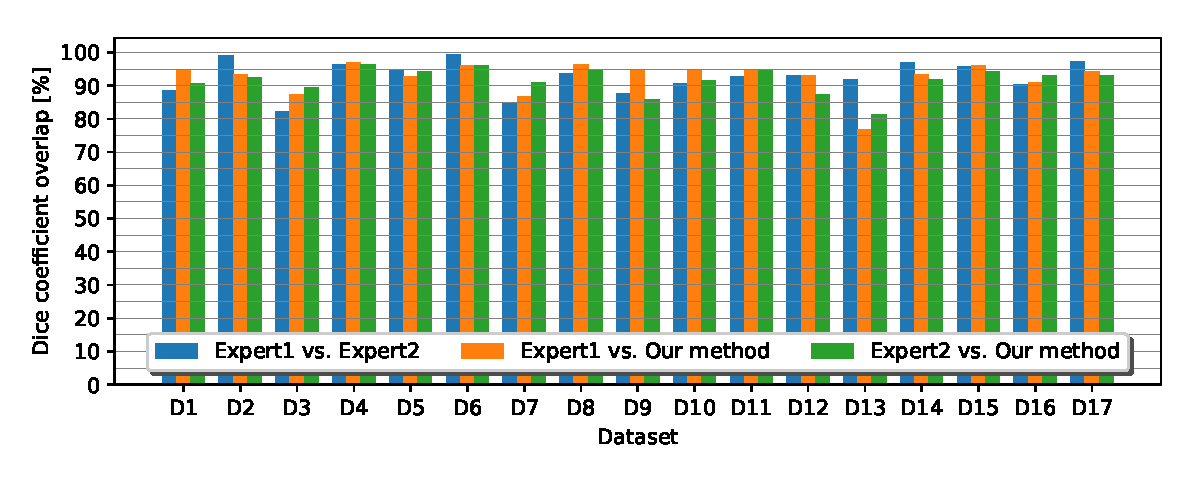
\includegraphics[width=\linewidth]{fig12.eps}
  % figure caption is below the figure
  \caption{Plot of dice coefficients overlap.}
  \label{fig:dices_plot}       % Give a unique label
\end{figure*}

\begin{figure*}[t]
  \centering
  % Use the relevant command to insert your figure file.
  % For example, with the graphicx package use
  \includegraphics[width=\linewidth]{fig13.png}
  % figure caption is below the figure
  \caption{Execution runtime of proposed method in each dataset. We use different color code for each step.
  }
  \label{fig:runtime_plot}       % Give a unique label
\end{figure*}

% For tables use
\begin{table}[t]
% table caption is above the table
  \centering
  \caption{Distance in mm between center points of our proposed
  location for LAA orifice and the desired location determined by 
  medical expert.} 
  \label{tab:cutdistances}
  % Give a unique label
% For LaTeX tables use
\begin{tabular}{ll} 
  \hline\noalign{\smallskip}
  Dataset & Distance in mm  \\
  \noalign{\smallskip}\hline\noalign{\smallskip}
  D1 & 0.00 mm \\
  D2 & 1.07 mm \\
  D3 & 5.84 mm \\
  D4 & 9.70 mm \\
  D5 & 0.53 mm \\
  D6 & 0.18 mm \\
  D7 & 1.62 mm \\
  D8 & 0.65 mm \\
  D9 & 4.04 mm \\
  D10 & 7.54 mm \\
  D11 & 0.50 mm \\
  D12 & 0.67 mm \\
  D13 & 0.57 mm \\
  D14 & 1.25 mm \\
  D15 & 0.00 mm \\
  D16 & 5.52 mm \\
  D17 & 3.07 mm \\
  Avg: & 2.51 mm \\
  \noalign{\smallskip}\hline
\end{tabular}
\end{table}




\begin{figure*}[]
  \centering
  \begin{subfigure}[]{.5\linewidth}
    \centering
    \includegraphics[width=\textwidth]{fig14topleft.png}
  \end{subfigure}%
  \begin{subfigure}[]{.5\linewidth}
    \centering
    \includegraphics[width=\textwidth]{fig14topright.png}
  \end{subfigure}%

  \begin{subfigure}[]{.5\linewidth}
    \centering
    \includegraphics[width=\textwidth]{fig14middleleft.png}
  \end{subfigure}%
  \begin{subfigure}[]{.5\linewidth}
    \centering
    \includegraphics[width=\textwidth]{fig14middleright.png}
  \end{subfigure}%

  \begin{subfigure}[]{.5\linewidth}
    \centering
    \includegraphics[width=\textwidth]{fig14bottomleft.png}
  \end{subfigure}%
  \begin{subfigure}[]{.5\linewidth}
    \centering
    \includegraphics[width=\textwidth]{fig14bottomright.png}
  \end{subfigure}%


  \caption{Segmentation results on 3 selected datasets. From left to right: our segmentation result (red), manual segmentation by the first expert (blue), manual segmentation by the second expert (green), plot of radius weighted rising
    slopes (on the right) and LAA delineation plane positions (our proposal in red and
  desired delineation plane in green). 
  }
  \label{fig:grounds_sidebyside}
\end{figure*}



Visualizations of several datasets segmented with the proposed method are
presented in Figure \ref{fig:segmentation_results}. Our segmentation results
are evaluated by dice similarity coefficient overlap with each of the two
validation datasets created by two medical experts. 
Our method achieves the average dice coefficient overlap of 92.52\% and 91.63\%
against the ground truth segmentations.  The average dice coefficient overlap
between the two ground truth segmentations is 92.66\%.  Results of the orifice
localization and minimum area cross-sectional plane placement are shown in
Figure \ref{fig:plane_dataset2}.  Our proposed LAA orifice localization is
evaluated against the desired location of the LAA orifice determined by the
expert. The average distance between our proposed location and the desired
location is 2.51 mm. 

The average runtime of our proposed segmentation method on our datasets is 
  two and a half  minutes (149 seconds 
on Intel i7, 4.3GHz, 16GB RAM).  
The runtime depends on the size of
the input dataset, as well as the anatomy of the patient in the dataset. The
execution runtimes for each dataset are presented in Figure
\ref{fig:runtime_plot}, where each step in the method is shown with different
color. Our method obtains clinically acceptable results.
                    
The delineation according to the calculated orifice location is performed for
both our segmentation and the ground truth expert segmentations. Table
\ref{tab:dices} shows the dice coefficient overlaps for each dataset.  Dice
overlaps are also shown in Figure \ref{fig:dices_plot} for easier
visualization.  Table \ref{tab:cutdistances} presents the distances in mm
between our proposed LAA orifice location and the desired LAA orifice location
determined by medical expert.  The results show that in most cases the desired
orifice location is either the location proposed by our method, or a location
very close to our proposed location. 



\section{Discussion}
\label{sec:discussion}

\begin{figure*}[t]
  \centering
  \begin{subfigure}[b]{.18\linewidth}
    \centering
    \includegraphics[width=\textwidth]{fig15_1.png}
    \caption{}
  \end{subfigure}%
  \begin{subfigure}[b]{.18\linewidth}
    \centering
    \includegraphics[width=\textwidth]{fig15_2.png}
    \caption{}
  \end{subfigure}%
  \begin{subfigure}[b]{.16\linewidth}
    \centering
    \includegraphics[width=\textwidth]{fig15_3.png}
    \caption{}
  \end{subfigure}%
  \begin{subfigure}[b]{.16\linewidth}
    \centering
    \includegraphics[width=\textwidth]{fig15_4.png}
    \caption{}
  \end{subfigure}%
  \begin{subfigure}[b]{.16\linewidth}
    \centering
    \includegraphics[width=\textwidth]{fig15_5.png}
    \caption{}\label{fig:siemens_b016}
  \end{subfigure}%
  \begin{subfigure}[b]{.16\linewidth}
    \centering
    \includegraphics[width=\textwidth]{fig15_6.png}
    \caption{}\label{fig:siemens_b011}
  \end{subfigure}%

  \caption{ Segmentation examples from LASC dataset and comparison to 
    SIE-PMB \cite{zheng2008_FourChamberHeartModeling} and SIE-MRG
    \cite{zheng2014_Multipartmodelingsegmentation}. Images show 
    our segmentation result (white), SIE-PMB (red) and SIE-MRG (green).
  }

  \label{fig:siemens}
\end{figure*}


  In this section we will discuss the comparison of the proposed method to the 
  other published state-of-the-art methods. Additionally, we will give 
  the practical implementation details of our
  proposed method and the reasoning behind certain choices of fixed parameter
  values. 

\subsection{Comparison to the state of the art}
  
  In addition to the direct comparison of the proposed method to the ground
  truth segmentations, we have compared the proposed method to two methods by
  \emph{Zheng et al.} (SIE-PMB \cite{zheng2008_FourChamberHeartModeling} and
  SIE-MRG \cite{zheng2014_Multipartmodelingsegmentation} from 
  \emph{Siemens Corporate Technology, Princeton, NJ, USA} -- SIE) on 20 datasets used
  in the Left Atrial Segmentation Challenge  (LASC)
  \cite{tobon-gomez2015_BenchmarkAlgorithmsSegmenting}.  The resulting
  segmentations were delineated from the LA by a plane determined by our
  medical expert. 
  The SIE methods  obtain the average dice
  overlap of 89.59\% between themselves, while our method obtains the average dice overlap of
  86.58\% and 86.26\% against the SIE-PMB and SIE-MRG, respectively.  Figure
  \ref{fig:siemens} shows the comparison of the segmentation results. Two of the
  SIE segmentation results in the LASC dataset had a part of the LAA removed during the 
  result standardization for LASC challenge (Figures \ref{fig:siemens_b016} and 
  \ref{fig:siemens_b011}),  affecting our dice overlap to their results negatively.
  If we remove those two datasets from the evaluation, the average dice overlap between the 
  SIE methods is 88.93\%, while our method obtains the average dice overlap of 
  87.29\% and 86.95\% against the SIE-PMB and SIE-MRG, respectively.
  
  LASC datasets are focused on the left atrium segmentation and the provided ground truth
  segmentations do not contain the LAA. Consequently, we were unable to compare 
  both our method and the SIE methods to the ground truth LAA segmentations.
  However, high overlap of our method to the SIE methods suggests that our method 
  can handle images of varying quality levels. The datasets in the LASC challenge were 
  specifically selected to provide a variety of quality levels: 8 high contrast,
  15 moderate contrast, 3 low contrast and 4 high noise datasets \cite{tobon-gomez2015_BenchmarkAlgorithmsSegmenting}.
  To the best of our knowledge, the two SIE methods are the only fully automatic
  LAA segmentation methods available.
  The SIE methods are very fast (SIE-MRG executes within 5 seconds), but
  require very large training samples (SIE-PMB was trained on 457 cardiac CT
  datasets). Our proposed method is completely heuristical and does not require
  any training.  

  The work proposed by \emph{Jin et al.} \cite{jin2018_LeftAtrialAppendage} uses 
  the fully convolutional neural networks (FCNs) combined with the 3D conditional 
  random fields to extract the LAA from the manually selected ROI. The method used 150
  datasets for training and evaluation and
  obtained the mean dice overlap of 94.76\%, while performing the segmentation in
  less than 40 seconds. The method is an improvement over the work by \emph{Wang et al.} 
  \cite{wang2016_LeftAtrialAppendage}, which
  obtains a slightly higher dice overlap (95.21\%), but requires more than 
  3.5 minutes of computation time.


\subsection{Method implementation details}

Our proposed method is robust to threshold value selection used to produce the
mask image. From the anatomical perspective, the method will correctly segment
the LAA even with a non-optimal threshold. 
Figure \ref{fig:grounds_sidebyside} shows the effect of the threshold
selection. The difference in segmentation between our two experts is a direct
result of the selected threshold value during the creation of the ground truth
images. 
  Depending on the selected threshold value, when the input image has high
  levels of noise, the resulting mask image can contain holes inside the LA
  near the LAA orifice. The presence of holes in the mask image can introduce
  errors in the maximum radius tracking step of the method and consequently the
  localization of the center of the LA. Thus, when working with very noisy
  images the user should select the threshold value which will minimize the
  appearance of holes in the mask image near the LAA orifice. The trabeculations
  inside the LAA do not impair the segmentation results.

\begin{figure*}[t]
  \centering
  \begin{subfigure}[b]{.6\linewidth}
    \centering
    \includegraphics[width=\textwidth]{fig16_legend.png}
  \end{subfigure}%


  \begin{subfigure}[b]{.18\linewidth}
    \centering
    \includegraphics[width=\textwidth]{fig16_1.png}
    \caption{}
  \end{subfigure}%
  \begin{subfigure}[b]{.17\linewidth}
    \centering
    \includegraphics[width=\textwidth]{fig16_2.png}
    \caption{}
  \end{subfigure}%
  \begin{subfigure}[b]{.18\linewidth}
    \centering
    \includegraphics[width=\textwidth]{fig16_3.png}
    \caption{}
  \end{subfigure}%
  \begin{subfigure}[b]{.16\linewidth}
    \centering
    \includegraphics[width=\textwidth]{fig16_4.png}
    \caption{}
  \end{subfigure}%
  \begin{subfigure}[b]{.11\linewidth}
    \centering
    \includegraphics[width=\textwidth]{fig16_5.png}
    \caption{}
  \end{subfigure}%
  \begin{subfigure}[b]{.21\linewidth}
    \centering
    \includegraphics[width=\textwidth]{fig16_6.png}
    \caption{}
  \end{subfigure}%

  \caption{ Visualization of the robustness of the method to seed point
    selection.  Each dot represents a different seed point. The color
    of the dot represents $\epsilon$ -- the absolute difference in dice overlap between
    the segmentation result obtained with that seed point and the ground truth. 
  }
  \label{fig:seeds_robustness}
\end{figure*}

The seed point selection is performed with a single click in a desired location
in the image. Optimally, the seed point should be placed deep in the LAA, near
the tip. 
  We have evaluated the robustness to the seed point selection
  by segmenting each dataset with a hundred randomly selected seed points (1700 evaluations). 
  The method achieves an average dice overlap of 87.74\% and 86.96\% against 
  the first and the second expert across all 1700 evaluations.
  The Figure \ref{fig:seeds_robustness} clearly shows how the distance of 
  the seed point from the orifice affects the segmentation results. 
  The dice overlap achieved in this test is relatively high, even though a large proportion
  of the randomly chosen seed points are very close to the orifice.
  When we ignore the half of the seed points closest to the orifice (obviously 
  incorrectly placed seed points), 
  the average dice overlaps with ground truths increase to 90.89\% and 90.23\%.
If the seed point is chosen too close to the atrium, it could happen that only
a smaller part of the appendage is segmented because the residual part of the
appendage may be too large (in comparison to the initial segmentation) to be
added to the final segmentation (see the segmentation refinement step in
Subsection~\ref{sec:final_seg}). However, selecting any seed point in the
deeper part of the appendage will result in the correct segmentation.

\begin{figure}[t]
  \centering
  \includegraphics[width=0.3\linewidth]{fig17.png}
  \caption{Clusters of voxels in the maximum radius path during maximum
  radius tracking. The voxels in the path will cluster at the center of 
  anatomical widenings before continuing the path towards the center of the 
  left atrium. The left atrium itself is among the  largest spherical areas in 
  the heart. The tracked path will stay in the LA center until the number of iterations 
  runs out.
} 
  \label{fig:centerline_clusters}       % Give a unique label
\end{figure}


The method for tracking maximum radii voxels (described in
Subsection~\ref{sec:centerline_path}) performs the search for the highest
radius voxel in the volume of the maximum inscribed spheres of all previously
tracked voxels.  
Our experiments have shown that using the 26-neighborhood
instead of the full spherical neighborhood
improves the performance of the method. 
The method is performed in a predefined
number of iterations (estimated from the image size, image spacing and expected
anatomical properties of the LAA) in which we are certain that the output set
$T$ will contain voxels from the central part of the atrium. The number of
iterations in our experiments is set to 4000 (which is larger than needed). In
most of our datasets the method detects the correct atrium location in well below
1000 iterations, while only two datasets take up to 1500 iterations. 
The two examples that need the most iterations have a large spherical widening in the 
anatomy. One of them is presented in the Figure \ref{fig:centerline_clusters}, with the 
output set $T$ in blue.
The voxels in $T$ will cluster in the center of such spherical widening, until
the next voxel with the largest radius is the voxel that will continue the path towards
the left atrium.
Red and green dashed circles in the figure show two largest spherical areas along
the path, one in the LAA (red) and the other in the LA (green). The voxels in the 
red circle will be discarded during centerline extraction 
(see also Figure \ref{fig:centerline_path}).
The center of the LA is extracted from the green cluster by finding the voxel
with the largest radius value and discarding all voxels added to $T$ after that voxel.
One possible limitation of our method is the case when the LAA has a large spherical part 
(similar to Figure \ref{fig:centerline_clusters}), but has a narrow neck. There is 
a possibility that the tracking method will run out of iterations before the path
$T$ enters the left atrium, thus failing to detect the centerline properly.
In this case we can allow the user to fix the detection by manually selecting
the second seed point inside the atrium, 
as shown in our earlier work \cite{leventic2017_SemiautomaticLeftAtrial}.


The search for the smallest cross-sectional area along the appendage centerline
is not performed along the whole centerline. At the point where the centerline
enters the atrium, the area significantly increases and varies due to the shape
of the atrium and its connected structures (vessels).  In order to avoid the
unneeded analysis of the cross-sections in the atrium (to improve speed and
accuracy of the computation), we define here criteria for choosing the
centerline position at which we stop the search for the minimal area.  We
observed that the maximum radius inside the LA is always at least twice as
large as the radius anywhere inside the LAA. Therefore, we stop the search for
minimal areas when the radius along the centerline becomes larger than half of
the maximum radius in the atrium.  The right side of Figure
\ref{fig:grounds_sidebyside} shows the plot of calculated areas $a(i)$ and
radius weighted rising slopes $w_r(i)$ for the visualized segmentation. 






\section{Conclusion}
\label{sec:conclusion}

We designed an effective semi-automatic method for segmentation of LAA from 3D
coronary CT angiography (CCTA) images and a novel orifice localization method
to aid the occluder placement procedure. The method requires two inputs from
the user: a threshold value and a seed point inside the LAA. The proposed
segmentation method is robust to segmentation leaks.  We introduced an approach
for extraction of LAA centerline, which is used in the further segmentation
steps.  Based on the extracted centerline, we introduced a new method for
localization of LAA orifice as the proposed location for placement of the
occluder device. The segmentation results were evaluated on ground truth images
from 17 CCTA datasets created by two medical experts. The obtained Dice
coefficient values indicate high correspondence to ground truth segmentations. 
Our results on proposed locations for the LAA occluder placement (orifice
localization) show high correlation to the preferred placement locations
determined by a medical expert.  The proposed methods yield clinically
acceptable results which indicate potential for use in the occluder placement
procedure planning. The designed application performs LAA measurements needed
to determine the appropriate size of the closure device while requiring little
manual intervention to perform the segmentation and analysis.

\subsection{Compliance with ethical standards}

\paragraph{\textbf{Conflict of Interest}} The authors declare that they have no
conflict of interest.

\paragraph{\textbf{Ethical approval}} For this type of study, formal consent is 
not required.

\paragraph{\textbf{Informed consent}} Informed consent was obtained from all
individual participants included in the study.

\subsection{Acknowledgments}
This work has been supported in part by Croatian Science Foundation under the project UIP-2017-05-4968.






\bibliographystyle{elsarticle-num}     

\begin{thebibliography}{10}
\expandafter\ifx\csname url\endcsname\relax
  \def\url#1{\texttt{#1}}\fi
\expandafter\ifx\csname urlprefix\endcsname\relax\def\urlprefix{URL }\fi
\expandafter\ifx\csname href\endcsname\relax
  \def\href#1#2{#2} \def\path#1{#1}\fi

\bibitem{worldhealthorganization2017_top10causes}
{World Health Organization}, The top 10 causes of death worldwide fact sheet,
  Tech. rep. (2017).

\bibitem{korhonen2015_LeftAtrialAppendage}
M.~Korhonen, A.~Muuronen, O.~Arponen, P.~Mustonen, M.~Hedman, P.~J\"ak\"al\"a,
  R.~Vanninen, M.~Taina, Left {{Atrial Appendage Morphology}} in {{Patients}}
  with {{Suspected Cardiogenic Stroke}} without {{Known Atrial Fibrillation}},
  PLOS ONE 10~(3) (2015) e0118822.
\newblock \href {http://dx.doi.org/10.1371/journal.pone.0118822}
  {\path{doi:10.1371/journal.pone.0118822}}.

\bibitem{budge2008_Analysisvivoleft}
L.~P. Budge, K.~M. Shaffer, J.~R. Moorman, D.~E. Lake, J.~D. Ferguson, J.~M.
  Mangrum, Analysis of in vivo left atrial appendage morphology in patients
  with atrial fibrillation: A direct comparison of transesophageal
  echocardiography, planar cardiac {{CT}}, and segmented three-dimensional
  cardiac {{CT}}, Journal of Interventional Cardiac Electrophysiology 23~(2)
  (2008) 87--93.
\newblock \href {http://dx.doi.org/10.1007/s10840-008-9281-7}
  {\path{doi:10.1007/s10840-008-9281-7}}.

\bibitem{blackshear1996_Appendageobliterationreduce}
J.~L. Blackshear, J.~A. Odell, Appendage obliteration to reduce stroke in
  cardiac surgical patients with atrial fibrillation, The Annals of Thoracic
  Surgery 61~(2) (1996) 755--759.
\newblock \href {http://dx.doi.org/10.1016/0003-4975(95)00887-X}
  {\path{doi:10.1016/0003-4975(95)00887-X}}.

\bibitem{goldman1999_Pathophysiologiccorrelatesthromboembolism}
M.~E. Goldman, L.~A. Pearce, R.~G. Hart, M.~Zabalgoitia, R.~W. Asinger,
  R.~Safford, J.~L. Halperin, S.~P. i. A.~F. Investigators, {others},
  Pathophysiologic correlates of thromboembolism in nonvalvular atrial
  fibrillation: {{I}}. {{Reduced}} flow velocity in the left atrial appendage
  ({{The Stroke Prevention}} in {{Atrial Fibrillation}} [{{SPAF}}-{{III}}]
  study), Journal of the American Society of Echocardiography 12~(12) (1999)
  1080--1087.

\bibitem{chugh2013_WorldwideEpidemiologyAtrial}
S.~S. Chugh, R.~Havmoeller, K.~Narayanan, D.~Singh, M.~Rienstra, E.~J.
  Benjamin, R.~F. Gillum, Y.-H. Kim, J.~H. McAnulty, Z.-J. Zheng, M.~H.
  Forouzanfar, M.~Naghavi, G.~A. Mensah, M.~Ezzati, C.~J.~L. Murray, Worldwide
  {{Epidemiology}} of {{Atrial Fibrillation}}: {{A Global Burden}} of
  {{Disease}} 2010 {{Study}}, Circulation (2013) CIRCULATIONAHA.113.005119\href
  {http://dx.doi.org/10.1161/CIRCULATIONAHA.113.005119}
  {\path{doi:10.1161/CIRCULATIONAHA.113.005119}}.

\bibitem{panaich2017_LeftAtrialAppendage}
S.~Panaich, J.~Holmes, David~R., Left {{Atrial Appendage Occlusion}} (2017).

\bibitem{holmes2015_LeftAtrialAppendage}
J.~Holmes, David~R., S.~K. Doshi, S.~Kar, M.~J. Price, J.~M. Sanchez,
  H.~Sievert, M.~Valderrabano, V.~Y. Reddy, Left {{Atrial Appendage Closure}}
  as an {{Alternative}} to {{Warfarin}} for {{Stroke Prevention}} in {{Atrial
  FibrillationA Patient}}-{{Level Meta}}-{{Analysis}}, Journal of the American
  College of Cardiology 65~(24) (2015) 2614--2623.
\newblock \href {http://dx.doi.org/10.1016/j.jacc.2015.04.025}
  {\path{doi:10.1016/j.jacc.2015.04.025}}.

\bibitem{reddy2013_LeftAtrialAppendage}
V.~Y. Reddy, S.~{M\"obius-Winkler}, M.~A. Miller, P.~Neuzil, G.~Schuler,
  J.~Wiebe, P.~Sick, H.~Sievert, Left {{Atrial Appendage Closure With}} the
  {{Watchman Device}} in {{Patients With}} a {{Contraindication}} for {{Oral
  Anticoagulation}}, Journal of the American College of Cardiology 61~(25)
  (2013) 2551--2556.
\newblock \href {http://dx.doi.org/10.1016/j.jacc.2013.03.035}
  {\path{doi:10.1016/j.jacc.2013.03.035}}.

\bibitem{saw2016_ComparingMeasurementsCT}
J.~Saw, P.~Fahmy, R.~Spencer, R.~Prakash, P.~Mclaughlin, S.~Nicolaou, M.~Tsang,
  Comparing {{Measurements}} of {{CT Angiography}}, {{TEE}}, and
  {{Fluoroscopy}} of the {{Left Atrial Appendage}} for {{Percutaneous
  Closure}}, Journal of Cardiovascular Electrophysiology 27~(4) (2016)
  414--422.
\newblock \href {http://dx.doi.org/10.1111/jce.12909}
  {\path{doi:10.1111/jce.12909}}.

\bibitem{goitein2017_CardiacCTAngiography}
O.~Goitein, N.~Fink, I.~Hay, E.~D. Segni, V.~Guetta, D.~Goitein, Y.~Brodov,
  E.~Konen, M.~Glikson, Cardiac {{CT Angiography}} ({{CCTA}}) predicts left
  atrial appendage occluder device size and procedure outcome, The
  International Journal of Cardiovascular Imaging 33~(5) (2017) 739--747.
\newblock \href {http://dx.doi.org/10.1007/s10554-016-1050-6}
  {\path{doi:10.1007/s10554-016-1050-6}}.

\bibitem{wunderlich2015_PercutaneousInterventionsLeft}
N.~C. Wunderlich, R.~Beigel, M.~J. Swaans, S.~Y. Ho, R.~J. Siegel, Percutaneous
  {{Interventions}} for {{Left Atrial Appendage Exclusion}}, JACC:
  Cardiovascular Imaging 8~(4) (2015) 472--488.
\newblock \href {http://dx.doi.org/10.1016/j.jcmg.2015.02.002}
  {\path{doi:10.1016/j.jcmg.2015.02.002}}.

\bibitem{cabrera2014_Leftatrialappendage}
J.~A. Cabrera, F.~Saremi, D.~{S\'anchez-Quintana}, Left atrial appendage:
  Anatomy and imaging landmarks pertinent to percutaneous transcatheter
  occlusion, Heart 100~(20) (2014) 1636--1650.
\newblock \href {http://dx.doi.org/10.1136/heartjnl-2013-304464}
  {\path{doi:10.1136/heartjnl-2013-304464}}.

\bibitem{song2016_MorphologicAssessmentLeft}
H.~Song, Q.~Zhou, Q.~Deng, J.~Chen, L.~Zhang, T.~Tan, R.~Guo, Morphologic
  {{Assessment}} of the {{Left Atrial Appendage}} in {{Patients}} with {{Atrial
  Fibrillation}} by {{Gray Values}}\textendash{{Inverted Volume}}-{{Rendered
  Imaging}} of {{Three}}-{{Dimensional Transesophageal Echocardiography}}: {{A
  Comparative Study}} with {{Computed Tomography}}, Journal of the American
  Society of Echocardiography 29~(11) (2016) 1100--1108.
\newblock \href {http://dx.doi.org/10.1016/j.echo.2016.08.003}
  {\path{doi:10.1016/j.echo.2016.08.003}}.

\bibitem{otton2015_LeftAtrialAppendage}
J.~M. Otton, R.~Spina, R.~Sulas, R.~N. Subbiah, N.~Jacobs, D.~W.~M. Muller,
  B.~Gunalingam, Left {{Atrial Appendage Closure Guided}} by {{Personalized
  3D}}-{{Printed Cardiac Reconstruction}}, JACC: Cardiovascular Interventions
  8~(7) (2015) 1004--1006.
\newblock \href {http://dx.doi.org/10.1016/j.jcin.2015.03.015}
  {\path{doi:10.1016/j.jcin.2015.03.015}}.

\bibitem{caselles1997_Geodesicactivecontours}
V.~Caselles, R.~Kimmel, G.~Sapiro, Geodesic active contours, International
  journal of computer vision 22~(1) (1997) 61--79.

\bibitem{yushkevich2006_Userguided3Dactive}
P.~A. Yushkevich, J.~Piven, H.~C. Hazlett, R.~G. Smith, S.~Ho, J.~C. Gee,
  G.~Gerig, User-guided {{3D}} active contour segmentation of anatomical
  structures: {{Significantly}} improved efficiency and reliability, NeuroImage
  31~(3) (2006) 1116--1128.
\newblock \href {http://dx.doi.org/10.1016/j.neuroimage.2006.01.015}
  {\path{doi:10.1016/j.neuroimage.2006.01.015}}.

\bibitem{babin2012_Generalizedpixelprofiling}
D.~Babin, A.~Pizurica, R.~Bellens, J.~De~Bock, Y.~Shang, B.~Goossens,
  E.~Vansteenkiste, W.~Philips, Generalized pixel profiling and comparative
  segmentation with application to arteriovenous malformation segmentation,
  Medical Image Analysis 16~(5) (2012) 991--1002, wOS:000306390300005.
\newblock \href {http://dx.doi.org/10.1016/j.media.2012.02.006}
  {\path{doi:10.1016/j.media.2012.02.006}}.

\bibitem{babin2013_Brainbloodvessel}
D.~Babin, A.~Pi{\v z}urica, J.~D. Vylder, E.~Vansteenkiste, W.~Philips, Brain
  blood vessel segmentation using line-shaped profiles, Physics in Medicine \&
  Biology 58~(22) (2013) 8041.
\newblock \href {http://dx.doi.org/10.1088/0031-9155/58/22/8041}
  {\path{doi:10.1088/0031-9155/58/22/8041}}.

\bibitem{zheng2008_FourChamberHeartModeling}
Y.~Zheng, A.~Barbu, B.~Georgescu, M.~Scheuering, D.~Comaniciu, Four-{{Chamber
  Heart Modeling}} and {{Automatic Segmentation}} for 3-{{D Cardiac CT Volumes
  Using Marginal Space Learning}} and {{Steerable Features}}, IEEE Transactions
  on Medical Imaging 27~(11) (2008) 1668--1681.
\newblock \href {http://dx.doi.org/10.1109/TMI.2008.2004421}
  {\path{doi:10.1109/TMI.2008.2004421}}.

\bibitem{zheng2014_Multipartmodelingsegmentation}
Y.~Zheng, D.~Yang, M.~John, D.~Comaniciu, Multi-part modeling and segmentation
  of left atrium in {{C}}-arm {{CT}} for image-guided ablation of atrial
  fibrillation, IEEE transactions on medical imaging 33~(2) (2014) 318--331.

\bibitem{jin2018_LeftAtrialAppendage}
C.~Jin, J.~Feng, L.~Wang, J.~Liu, H.~Yu, J.~Lu, J.~Zhou, Left {{Atrial
  Appendage Segmentation Using Fully Convolutional Neural Networks}} and
  {{Modified Three}}-dimensional {{Conditional Random Fields}}, IEEE Journal of
  Biomedical and Health Informatics PP~(99) (2018) 1--1.
\newblock \href {http://dx.doi.org/10.1109/JBHI.2018.2794552}
  {\path{doi:10.1109/JBHI.2018.2794552}}.

\bibitem{wang2016_LeftAtrialAppendage}
L.~Wang, J.~Feng, C.~Jin, J.~Lu, J.~Zhou, Left {{Atrial Appendage Segmentation
  Based}} on {{Ranking}} 2-{{D Segmentation Proposals}}, in: Statistical
  {{Atlases}} and {{Computational Models}} of the {{Heart}}. {{Imaging}} and
  {{Modelling Challenges}}, {Springer, Cham}, 2016, pp. 21--29.
\newblock \href {http://dx.doi.org/10.1007/978-3-319-52718-5_3}
  {\path{doi:10.1007/978-3-319-52718-5_3}}.

\bibitem{jin2017_LeftAtrialAppendage}
C.~Jin, H.~Yu, J.~Feng, L.~Wang, J.~Lu, J.~Zhou, Left {{Atrial Appendage Neck
  Modeling}} for {{Closure Surgery}}, in: Statistical {{Atlases}} and
  {{Computational Models}} of the {{Heart}}. {{ACDC}} and {{MMWHS Challenges}},
  Lecture Notes in Computer Science, {Springer, Cham}, 2017, pp. 32--41.
\newblock \href {http://dx.doi.org/10.1007/978-3-319-75541-0_4}
  {\path{doi:10.1007/978-3-319-75541-0_4}}.

\bibitem{jin2018_Leftatrialappendagea}
C.~Jin, J.~Feng, L.~Wang, H.~Yu, J.~Liu, J.~Lu, J.~Zhou, Left atrial appendage
  segmentation and quantitative assisted diagnosis of atrial fibrillation based
  on fusion of temporal-spatial information, Computers in Biology and Medicine
  96 (2018) 52--68.
\newblock \href {http://dx.doi.org/10.1016/j.compbiomed.2018.03.002}
  {\path{doi:10.1016/j.compbiomed.2018.03.002}}.

\bibitem{grasland-mongrain2009_Segmentationleftatrial}
P.~{Grasland-Mongrain}, Segmentation of the left atrial appendage from {{3D}}
  images, Ph.D. thesis, Master Thesis. ENS Cachan (2009).

\bibitem{grasland-mongrain2010_Combinationshapeconstrainedinflation}
P.~{Grasland-Mongrain}, J.~Peters, O.~Ecabert, Combination of shape-constrained
  and inflation deformable models with application to the segmentation of the
  left atrial appendage, in: Biomedical {{Imaging}}: {{From Nano}} to
  {{Macro}}, 2010 {{IEEE International Symposium}} On, {IEEE}, 2010, pp.
  428--431.

\bibitem{zhong2012_Segmentationremovalpulmonary}
H.~Zhong, Y.~Zheng, G.~{Funka-Lea}, F.~{Vega-Higuera}, Segmentation and removal
  of pulmonary arteries, veins and left atrial appendage for visualizing
  coronary and bypass arteries, in: Computer {{Vision}} and {{Pattern
  Recognition Workshops}} ({{CVPRW}}), 2012 {{IEEE Computer Society
  Conference}} On, {IEEE}, 2012, pp. 24--30.

\bibitem{zhong2013_Automaticheartisolation}
H.~Zhong, Y.~Zheng, G.~{Funka-Lea}, F.~{Vega-Higuera}, Automatic heart
  isolation in {{3D CT}} images, in: Medical {{Computer Vision}}. {{Recognition
  Techniques}} and {{Applications}} in {{Medical Imaging}}, {Springer}, 2013,
  pp. 165--180.

\bibitem{leventic2017_SemiautomaticLeftAtrial}
H.~Leventi\'c, D.~Babin, L.~Velicki, I.~Gali\'c, V.~Zlokolica, Semi-automatic
  {{Left Atrial Appendage Segmentation}} from {{3D CCTA}} images, in:
  Proceedings {{ELMAR}}-2017, {IEEE}, Zadar, Croatia, 2017, pp. 39--42.

\bibitem{maurer2003_LinearTimeAlgorithm}
C.~R. Maurer, Jr., R.~Qi, V.~Raghavan, A {{Linear Time Algorithm}} for
  {{Computing Exact Euclidean Distance Transforms}} of {{Binary Images}} in
  {{Arbitrary Dimensions}}, IEEE Trans. Pattern Anal. Mach. Intell. 25~(2)
  (2003) 265--270.
\newblock \href {http://dx.doi.org/10.1109/TPAMI.2003.1177156}
  {\path{doi:10.1109/TPAMI.2003.1177156}}.

\bibitem{lowekamp2013_DesignSimpleITK}
B.~C. Lowekamp, D.~T. Chen, L.~Ib\'a\~nez, D.~Blezek, The {{Design}} of
  {{SimpleITK}}, Frontiers in Neuroinformatics 7.
\newblock \href {http://dx.doi.org/10.3389/fninf.2013.00045}
  {\path{doi:10.3389/fninf.2013.00045}}.

\bibitem{babin2018_Skeletonizationmethodvessel}
D.~Babin, A.~Pi{\v z}urica, L.~Velicki, V.~Mati\'c, I.~Gali\'c, H.~Leventi\'c,
  V.~Zlokolica, W.~Philips, Skeletonization method for vessel delineation of
  arteriovenous malformation, Computers in Biology and Medicine 93 (2018)
  93--105.
\newblock \href {http://dx.doi.org/10.1016/j.compbiomed.2017.12.011}
  {\path{doi:10.1016/j.compbiomed.2017.12.011}}.

\bibitem{dijkstra1959_notetwoproblems}
E.~W. Dijkstra, A note on two problems in connexion with graphs, Numerische
  Mathematik 1~(1) (1959) 269--271.
\newblock \href {http://dx.doi.org/10.1007/BF01386390}
  {\path{doi:10.1007/BF01386390}}.

\bibitem{walker2012_Anatomicalanalysisleft}
D.~T. Walker, J.~A. Humphries, K.~P. Phillips, Anatomical analysis of the left
  atrial appendage using segmented, three-dimensional cardiac {{CT}}: A
  comparison of patients with paroxysmal and persistent forms of atrial
  fibrillation, Journal of Interventional Cardiac Electrophysiology 34~(2)
  (2012) 173--179.
\newblock \href {http://dx.doi.org/10.1007/s10840-011-9638-1}
  {\path{doi:10.1007/s10840-011-9638-1}}.

\bibitem{christiaens2010_Realthreedimensionalassessment}
L.~Christiaens, N.~{Varroud-Vial}, P.~Ardilouze, S.~Ragot, J.~Mergy, B.~Bonnet,
  D.~Herpin, J.~Allal, Real three-dimensional assessment of left atrial and
  left atrial appendage volumes by 64-slice spiral computed tomography in
  individuals with or without cardiovascular disease, International Journal of
  Cardiology 140~(2) (2010) 189--196.
\newblock \href {http://dx.doi.org/10.1016/j.ijcard.2008.11.055}
  {\path{doi:10.1016/j.ijcard.2008.11.055}}.

\bibitem{tobon-gomez2015_BenchmarkAlgorithmsSegmenting}
C.~{Tobon-Gomez}, A.~J. Geers, J.~Peters, J.~Weese, K.~Pinto, R.~Karim,
  M.~Ammar, A.~Daoudi, J.~Margeta, Z.~Sandoval, B.~Stender, Y.~Zheng, M.~A.
  Zuluaga, J.~Betancur, N.~Ayache, M.~A. Chikh, J.~Dillenseger, B.~M. Kelm,
  S.~Mahmoudi, S.~Ourselin, A.~Schlaefer, T.~Schaeffter, R.~Razavi, K.~S.
  Rhode, Benchmark for {{Algorithms Segmenting}} the {{Left Atrium From 3D CT}}
  and {{MRI Datasets}}, IEEE Transactions on Medical Imaging 34~(7) (2015)
  1460--1473.
\newblock \href {http://dx.doi.org/10.1109/TMI.2015.2398818}
  {\path{doi:10.1109/TMI.2015.2398818}}.

\end{thebibliography}




\end{document}

